%Dies ist die Hauptseite des Dokumentes. Es werden u. a. alle Kapitel,
% Einstellung im Header eingebunden.
%Ver�nderungen m�ssen in folgenden Dateien vorgenommen werden:
			%- Layout.tex 
			%- newComments.tex
			%- Titelseite
			%- Versions�bersicht
			%- einzelne Kapitel (evtl. erweitern) 
			
% Definition von globalen Parametern, die derzeit auf der Titelseite und in der Kopfzeile 
% verwendet werden. Der in <> gesetzte Text ist zu ver�ndern.  

\newcommand{\praktikumTitel}{<Titel des Praktikums>}
\newcommand{\projektTitel}{<Titel des Teilprojektes>}


%Hier sind alle Einstellungen enthalten, die sich auf das Seiten- und Dokumentenlayout beziehen

\documentclass[
	11pt,								% Schriftgr��e
	DIV12,
	german,							% f�r Umlaute, Silbentrennung etc.
	oneside,						% einseitiges Dokument
	titlepage,					% es wird eine Titelseite verwendet
	halfparskip,				% Abstand zwischen Abs�tzen (halbe Zeile)
	normalheadings,			% Gr��e der �berschriften verkleinern
	tablecaptionabove,	% Beschriftung von Tabellen unterhalb ausgeben
	final								% Status des Dokuments (final/draft)
]{scrreprt}						% 


%------�ndern von Schriftschnitten - (Muss ganz am Anfang stehen !) -------------
\usepackage{fix-cm}

%------Umlaute ------------------------------------------------------------------
% 	Umlaute/Sonderzeichen wie ���� k�nnen direkt im Quelltext verwenden werden.
%		Erlaubt automatische Trennung von Worten mit Umlauten.
\usepackage[T1]{fontenc}								 
\usepackage[latin1]{inputenc}

%------Anpassung der Landessprache-----------------------------------------------
\usepackage{ngerman}

%------Einfache Definition der Zeilenabst�nde und Seitenr�nder-------------------
\usepackage{geometry}
\usepackage{setspace}
\usepackage{tocbasic}

%------Schriftgr��enanpassung von einzelnen Textpassagen-------------------------
\usepackage{relsize}

%------Trennlinien in Kopf- und Fusszeile
\usepackage[headsepline, footsepline, ilines]{scrpage2}

%------Grafiken------------------------------------------------------------------
\usepackage{graphicx}
\usepackage{float}

%------Packet zum Sperren, Unterstreichen und Hervorheben von Texten------------
\usepackage{soul}

%------erg�nzende Schriftart----------------------------------------------------
\usepackage{helvet}

%------Lange Tabellen-----------------------------------------------------------
\usepackage{longtable}
\usepackage{array}
\usepackage{ragged2e}
\usepackage{lscape}

\usepackage{xparse}
\usepackage{framed}
\usepackage[usenames,dvipsnames]{color}

%------PDF-Optionen-------------------------------------------------------------
\usepackage[
	bookmarks,
	bookmarksopen=true,
	colorlinks=true,
	linkcolor=black,				% einfache interne Verkn�pfungen
	anchorcolor=black,			% Ankertext
	citecolor=black, 				% Verweise auf Literaturverzeichniseintr�ge im Text
	filecolor=black, 				% Verkn�pfungen, die lokale Dateien �ffnen
	menucolor=black, 				% Acrobat-Men�punkte
	urlcolor=black, 				% Farbe f�r URL-Links
	backref,								% Zur�cktext nach jedem Bibliografie-Eintrag als Liste von �berschriftsnummern
	pagebackref,						% Zur�cktext nach jedem Bibliografie-Eintrag als Liste von Seitenzahlen
	plainpages=false,				% zur korrekten Erstellung der Bookmarks
	pdfpagelabels,					% zur korrekten Erstellung der Bookmarks
	hypertexnames=false,		% zur korrekten Erstellung der Bookmarks
	% linktocpage 						% Seitenzahlen anstatt Text im Inhaltsverzeichnis verlinken
	]{hyperref}



			% enth�lt eingebundene Packete

%------Seitenr�nder-------------------------------------------------------------
\geometry{verbose, 										% zeigt die eingestellten Parameter beim Latexlauf an
			paper=a4paper, 									% Papierformat			
			top=25mm, 											% Rand oben
			left=25mm, 											% Rand links
			right=25mm, 										% Rand rechts
			bottom=45mm, 										% Rand unten
			pdftex													% schreibt das Papierformat in dei Ausgabe damit Ausgabeprogramm Papiergr��e erkennt		
	} 
	
%Seitenlayout
\onehalfspace        % 1,5-facher Abstand  

%------Kopf- und Fu�zeilen ------------------------------------------------------
\pagestyle{scrheadings}

%------Kopf- und Fu�zeile auch auf Kapitelanfangsseiten -------------------------
\renewcommand*{\chapterpagestyle}{scrheadings}

%------Schriftform der Kopfzeile ------------------------------------------------
\renewcommand{\headfont}{\normalfont}

%------Kopfzeile-----------------------------------------------------------------
\setlength{\headheight}{21mm}				% H�he der Kopfzeile
\ihead{\large{\textsc{\praktikumTitel}}\\		% Text in der linken Box
			 \small{\projektTitel}}
\chead{}														% Text in der mittleren Box

%----Fusszeile
\cfoot{}														% Text in mittlerer Box
\ofoot{\pagemark}										% Seitenzahl in rechter Box			





					% Diese Datei enth�lt alle Layouteinstellungen

%------Beginn des Gesamtdokumentes--------------------------------------------------------
\usepackage[american]{babel}
\usepackage{listings}
\usepackage{hyperref}
\begin{document}
\shorthandoff{"}
%------Eingebundene Seiten, Verzeichnisse bzw. Kapitel------------------------------------
%----Stil dieser Seite--------------------------------------------------------------------
\thispagestyle{plain}			% Kopfzeile bleibt leer

%----Beginn der Titelseite----------------------------------------------------------------
\begin{titlepage}

%----zentrierte Ausrichtung �ber die gesamte Seite----------------------------------------		
\begin{center}

%----Titel des Praktikum (\praktikumTitel in newComments zu ver�ndern)--------------------
{\relsize{4}{\textbf{\textsc{\praktikumTitel}}}}\\[5ex]

%----Titel des Teilprojektes (\projektTitel in newComments ver�ndern)---------------------
{\relsize{3}{\textbf{\textsc{\projektTitel}}}}\\[5ex]

Praxis der Softwarentwicklung\\
Summerterm 2014\\[6ex]

{\relsize{3}\so{\textbf{Softwaredesign}}}\\[5ex]

%----Titelbild------------------------------------------------------------

\includegraphics[scale=0.25]{bilder/logo.png}\\[5ex]

%----Daten des Auftraggebers
Client\\[2ex]															
KIT - Karlsruher Institut f�r Technologie\\
Fakult�t f�r Informatik\\										
Institut f�r Anthropromatik und Robotik (IAR)\\
Intelligente Prozessautomation und Robotik (IPR)\\[2ex]
Advisor: Andreas Bihlmaier\\
andreas.bihlmaier@gmx.net\\[5ex]

% ----Tabelle Teilnehmer---------------------------------------------------
Contributors\\

\begin{tabular}{l<{\hspace{20mm}} l<{\hspace{30mm}}}\\	
	Name 									& 	E-Mail-address\\			% Zeilen�berschift
		
	\hline										% Linie unterhalb der Zeilen�berschrift
	
	%----Nachfolgend alle Namen und E-Mail-Adressen der Teilnehmer einf�gen	
	Alex Weber & alex.weber3@gmx.net\\
	Matthias Hadlich & matthias.hadlich@student.kit.edu\\
	Matthias Klatte	& matthias.klatte@go4more.de\\
	Micha Wetzel & micha.wetzel@student.kit.edu\\	
	Sebastian Kneipp &	sebastian.kneipp@gmx.net
	
	
\end{tabular}\\[2ex]

\end{center}

\vfill Karlsruhe, 07.06.2014

\end{titlepage}
											% Titelseite	
\tableofcontents													% Inhaltsverzeichnis wird automatisch generiert
\newpage
% \listoffigures														% ebenso das Abbildungsverzeichnis

\include{content/introduction}
\chapter{Composition}

\section{Architecture}

\begin{figure}[here]
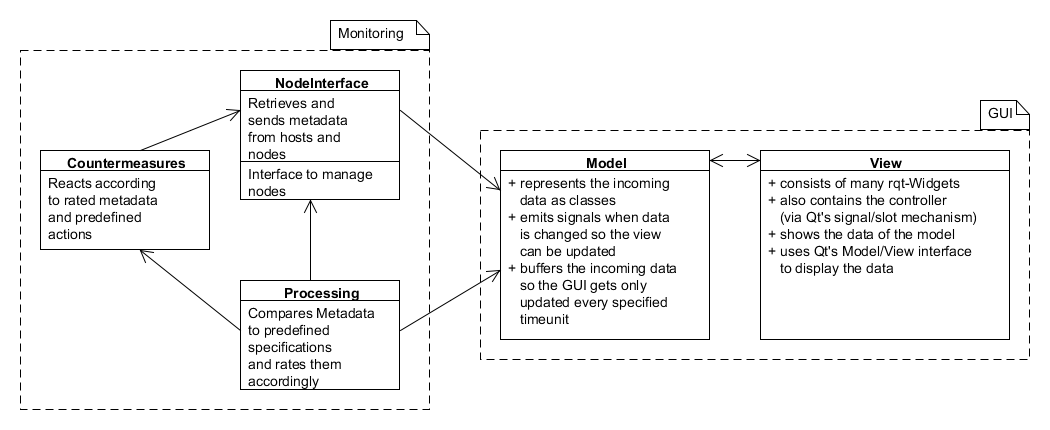
\includegraphics[width=\linewidth]{./bilder/architektur.png}
\caption{architecture}
\label{fig:architecture}
\end{figure}

Figure ~\ref{fig:architecture} shows the general architecture of our software. It is divided into two parts, one for the graphical user interface and one for the monitoring aspect.
The right part depicts the GUI. It is designed using the Qt MVC architecture, consisting of only two elements because Qt takes care of the controller: model and view. It will handle user-interaction.
The left part depicts the monitoring aspect. It consists of three elements : NodeInterface, Countermeasure and Processing. It will take care of collecting metadata, processing it and taking appropriate action in case of an error.

\subsection{Monitoring}

\begin{description}
	\item[NodeInterface] \mbox{}
		\begin{itemize}
			\item Retrieves and sends metadata from hosts and nodes
			\item Interface to manage nodes
		\end{itemize}
	\item[Processing] \mbox{} 
	Compares Metadata to predefined specifications and
	rates the accordingly
	\item[Countermeasures] \mbox{} 
	Reacts according to rated metadata and
	predefined actions
\end{description}

\subsection{GUI}

\begin{description}
	\item[Model] \mbox{}	
		\begin{itemize}
		\item Represents the incoming data as classes
		\item Emits signals when data is changed so the view can be updated
		\item Buffers the incoming data so the GUI gets only updated every specified timeunit
		\end{itemize}
	\item[View] \mbox{}
		\begin{itemize}
		\item Consists of many rqt-Widgets
		\item Also contains the controller (via Qt's signal/slot mechanism)
		\item Shows the data of the model
		\item Uses Qt's Model/View interface to display the data
		\item Also uses pyqtgraph to dynamically plot the incoming data
		\end{itemize}
\end{description}	
\chapter{Classes Description}

\section{Processing}

\subsection{MonitoringNode}
Main Class wrapping the processing functionality.

\subsubsection{Attributes}
\begin{itemize}
	\item private MetadataStorage storage
	\item private SpecificationHandler specHandler
\end{itemize}
\subsubsection{Methods}
\begin{itemize}
	\item \textbf{private Metadata receive\_data()}\\
	Receives data incoming from the Subscriber and converts them to Metadata objects.
	\item \textbf{private RatedStatistics process\_data(Metadata)}\\
	Returns the specHandler's compare result
	\item \textbf{private void publish\_data(RatedStatistics)}\\
	Publishes results of the comparison as rated Metadata
	\item \textbf{private MetadataStorageResponse storage\_server(MetadataStorageRequest)}\\
	Listen for the GUI Model service calls and returns requested metadata from the storage
\end{itemize}


\subsection{MetadataStorage}
Saves recieved metadata packages for a given period of time and can provide them on request.

\subsubsection{Attributes}
\begin{itemize}
	\item \textbf{private dict(string, dict(int, StorageContainer[])) storage}\\
	Datastructure to store Packages by key and timestamp
	\item \textbf{private int duration}\\
	Duration in seconds for data to be stored
\end{itemize}
\subsubsection{Methods}
\begin{itemize}
	\item \textbf{private void clean\_up()}\\
	Deletes Metadata exceeding the duration to store
	\item \textbf{public boolean store(StorageContainer)}\\
	Stores a given Metadata
	\item \textbf{public StorageContainer[] get(string, int)}\\
	Returns all Metadata packages for the given connection/host of the given amount of time.
	\item \textbf{public boolean clear()}\\
	Clears the whole storage
\end{itemize}


\subsection{StorageContainer}
Wraps Metadata in raw and rated form with an identifier and a timestamp. Object to be returned on request by the GUI model.

\subsubsection{Attributes}
\begin{itemize}
	\item \textbf{public int timestamp}\\
	Time when the data came from the subscriber
	\item \textbf{public string identifier}\\
	Host/Node/Connection identifier
	\item \textbf{public object data\_raw}\\
	The data as it reaches the subscriber from nodes and hosts.
	\item \textbf{public object data\_rated}\\
	The data like it would be published after being rated.
\end{itemize}


\subsection{Metadata}
Wraps metadata of exactly one host or node, a topic or a node-topic-combination.

\subsubsection{Attributes}
\begin{itemize}
	\item \textbf{private MetadataTuple[] values}\\
	Collection of Metadata regarding multiple meassurements.
\end{itemize}
\subsubsection{Methods}
\begin{itemize}
	\item \textbf{public void add\_tuple(MetadataTuple)}\\
	Add a MetadataTuple of information to the bundle.
	\item \textbf{public object get(String)}\\
	Returns the value of the MetadataTuple with the given key. False, if the key does not exist.
\end{itemize}


\subsection{Specification}
An object loaded from the specification configurations and basis for comparison of Metadata with desired values.

\subsubsection{Attributes}
\begin{itemize}
	\item \textbf{private MetadataTuple[] values}\\
	Collection of MetadataTuple objects providing limits for multiple fields.
\end{itemize}
\subsubsection{Methods}
\begin{itemize}
	\item \textbf{public void add\_tuple(MetadataTuple)}\\
	Adds a MetadataTuple to the bundle
	\item \textbf{public Object get(String)}\\
	Returns the value of the MetadataTuple with the given key. The returned value would be a list containing limit values for the most measured fields. False, if the key does not exist.
\end{itemize}


\subsection{SpecificationHandler}
Loads the specifications from the parameter server and compares them to the actual metadata.

\subsubsection{Attributes}
\begin{itemize}
	\item \textbf{private Specification[] specifications}\\
	Datastructure to keep all loaded Specification objects
\end{itemize}
\subsubsection{Methods}
\begin{itemize}
	\item \textbf{private void load\_specifications()}\\
	Loads the specifications from configuration files into Specification objects and stores them
	\item \textbf{public RatedStatistics compare(Metadata, Specification)}\\
	Compares a given Metadata object with a given Specification object regarding all available fields. Returns a RatedStatistics object wrapping potential divergences.
\end{itemize}


\subsection{RatedStatistics}
Wraps the result of the comparison between the actual metadata and the specificaton.

\subsubsection{Attributes}
\begin{itemize}
	\item \textbf{public string seuid}\\
	Identifies the node/host/connection
	\item \textbf{public string[] metatype}\\
	The metadata that was out of bounds
	\item \textbf{public string[] actual}\\
	The actual values
	\item \textbf{public string[] expected}\\
	The expected values
	\item \textbf{public int[] state}\\
	State of the metadata from the node/host/connection : state: { 0 = high ; 1 = low ; 2 = unknown}
\end{itemize}


\subsection{MetadataTuple}
Stores any kind of value for a certain key. Specifications storing values indicating limits, Metadata storing absolute actual values.

\subsubsection{Attributes}
\begin{itemize}
	\item private String key
	\item private Object value
\end{itemize}
\subsubsection{Methods}
\begin{itemize}
	\item public String get\_key()
	\item public Object get\_value()
\end{itemize}

% -----------------------------------------------------------------------------------
\section{NodesInterface}

\subsection{HostStastistic}
Singleton per host which contains statistics about the host and nodes running on the it. Handles request regarding node management.

\subsection{NodeManager}
Is able to stop or restart nodes.


% -----------------------------------------------------------------------------------
\newpage
\section{Countermeasure}
\begin{figure}[!ht]
\begin{center}
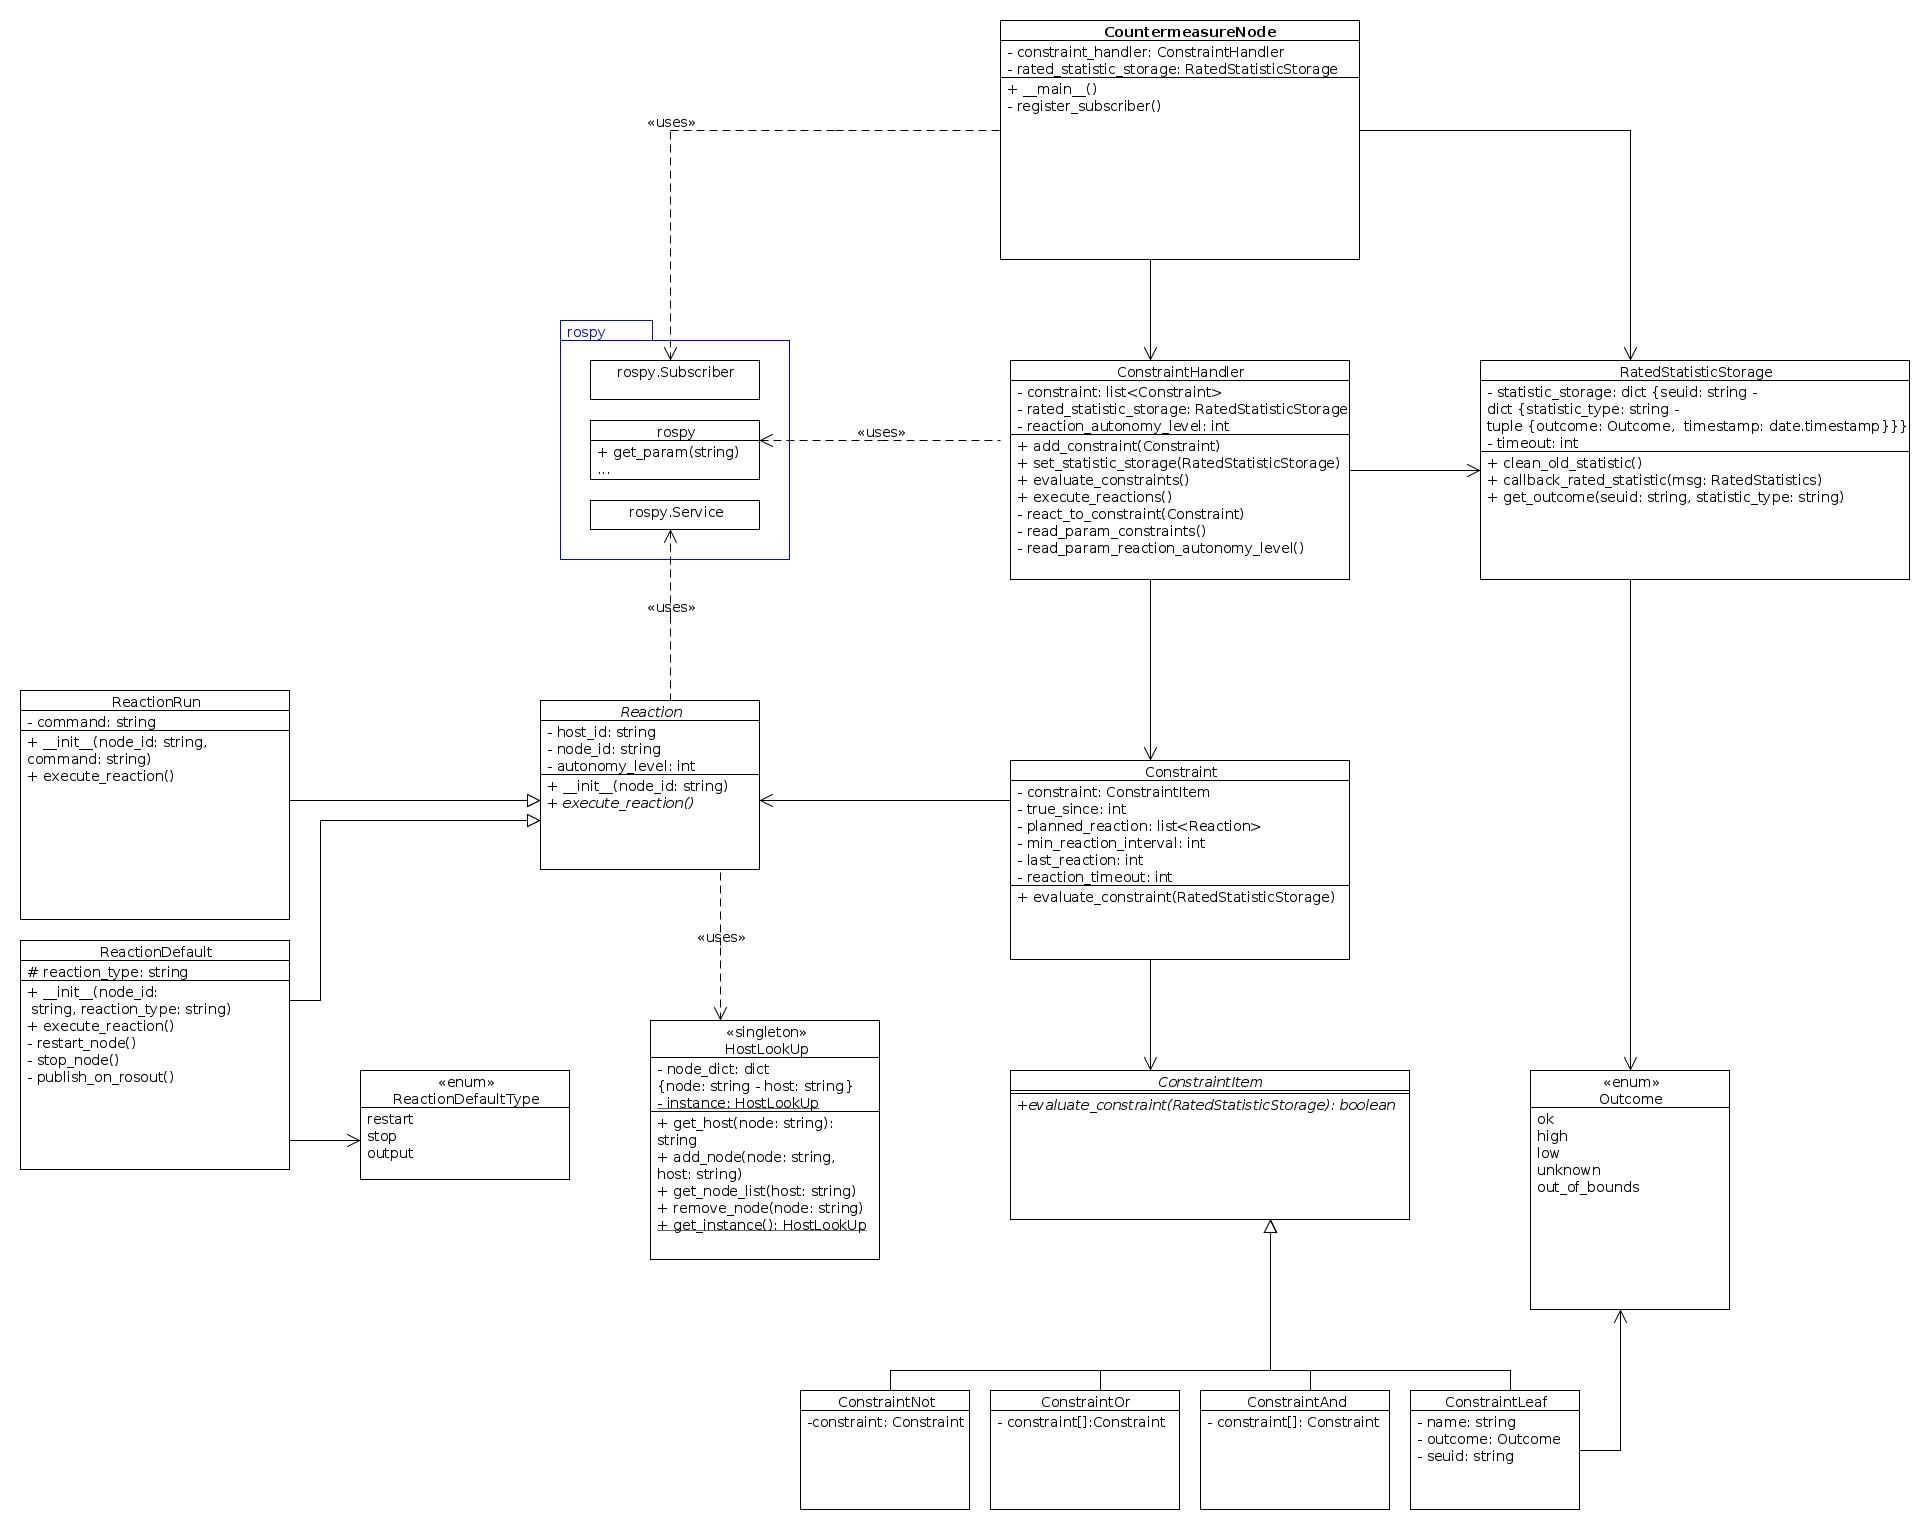
\includegraphics[width=1.0\linewidth]{./diagram_pictures/reactor.jpg}
\caption{The UML diagram of the countermeasure package}
\end{center}
\end{figure}

\mbox{}

\newpage


\subsection{CountermeasureNode}
a ROS node. Evaluates incoming rated statistics with a list of constraints. If those constraints turn out to be true appropriate action is taken.
\subsubsection{Attributes}
\begin{itemize}
	\item \textbf{ private ConstraintHandler constraint\_handler}\\
		the handler for all constraints
	\item \textbf{ private RatedStatisticStorage rated\_statistic\_storage}\\
		the storage of all incoming rated statistic
\end{itemize}
\subsubsection{Methods}
\begin{itemize}
	\item \textbf{ public void \_\_main\_\_() }\\\\
		periodically (threads) evaluates the constraints and cleans old statistics
	\item \textbf{ private void register\_subscriber() }\\
		registers to the rated statistics
\end{itemize}



\subsection{ConstraintHandler}
Manages all constraints, checks if they are true and executes appropriate reactions if neccessary.

\subsubsection{Attributes}
\begin{itemize}
	\item \textbf{ private list<Constraint> constraint }\\
		contains a list of all constraints
	\item \textbf{ private  RatedStatisticStorage rated\_statistic\_storage }\\
		contains all incoming rated statistic
	\item \textbf{ private  int reaction\_autonomy\_level }\\
		only reactions with an autonomy\_level <= reaction\_autonomy\_level get executed
\end{itemize}
\subsubsection{Methods}
\begin{itemize}
	\item \textbf{ public void add\_constraint(Constraint)  }\\
		adds an constraint to this list
	\item \textbf{ public void set\_statistic(RatedStatisticStorage)  }\\
		sets the Statistic to use. Should only be needed on initialisation
	\item \textbf{ public void evaluate\_constraints()  }\\
		evaluates every constraint
	\item \textbf{ public void execute\_reactions()  }\\
		checks if there are any new reactions to do and executes them.
	\item \textbf{ private void react\_to\_constraint(Constraint)  }\\
		executes an single Reaction and updates the attributes of the Constraint
	\item \textbf{ private void read\_param\_constraints()  }\\
		reads all constraints from the parameter server
	\item \textbf{ private void read\_param\_reaction\_autonomy\_level()  }\\
		reads the reaction\_autonomy\_level from the parameter server
\end{itemize}


\subsection{RatedStatisticStorage}
A database which contains the current state of all rated statistics.
\subsubsection{Attributes}
\begin{itemize}
	\item \textbf{ private dict\{string seuid - dict\{string statistic\_type - tuple\{Outcome outcome,date.timestamp timestamp\}\}\} statistic\_dict }\\
		a dictionary containing all rated statistic information with their outcome and an timestamp when they got added / updated to the dictionary.
	\item \textbf{ private int timeout }\\
		the timeout after which an item in ratedstatistic is declared too old and should be removed from the dict.
\end{itemize}
\subsubsection{Methods}
\begin{itemize}
	\item \textbf{ public void clean\_old\_statistic() }\\
		checks the complete dictionary for statistics older than timeout seconds and removes them.
	\item \textbf{ public void callback\_rated\_statistic(RatedStatistics msg) }\\
		callback for incoming rated statistics. adds them to the dictionary or removes items from the dictionary if the rated statistic says that its within bounds again. 
	\item \textbf{ public Outcome get\_outcome(string seuid, string statistic\_type) }\\
		returns the outcome of the specific seuid and statistic\_type.
\end{itemize}

\subsection{Constraint }
contains the whole constraint with corresponding reactions.


\subsubsection{Attributes}
\begin{itemize}
	\item \textbf{ private ConstraintItem constraint }\\
	first constraint in the chain of ConstraintItems.
	\item \textbf{ private int true\_since }\\
	epoch time in milliseconds since the constraint is true,
	if the constraint is not true it is 0
	\item \textbf{ private list<Reaction> planned\_reaction }\\
	an list of reactions that should be executed if the constraint has been true longer than min\_reaction\_interval milliseconds
	\item \textbf{ private int min\_reaction\_interval }\\
	the minimum time needed in ms that the constraint needs to be true to execute the planned\_reaction
	\item \textbf{ private int last\_reaction }\\
	contains the epoch time in ms when the reaction corresponding to this constraint has been executed for the last time.
		is 0 if it has never been executed
	\item \textbf{ private int reaction\_timeout }\\
	minimum durotation in ms needed before an reaction can happen again
\end{itemize}
\subsubsection{Methods}
\begin{itemize}
	\item \textbf{ public void evaluate\_constraint(RatedStatisticStorage)  }\\
	evaluates this constraint and sets the attributes according to the result of the evaluation
\end{itemize}



\subsection{ConstraintItem}
	Abstract description of a Constraint, can be an logical operation on constraints or an actual constraint
\subsubsection{Attributes}
\subsubsection{Methods}
\begin{itemize}
	\item \textbf{ public abstract boolean evaluate\_constraint(RatedStatisticStorage) }\\
	evaluates if this constraint, given the available RatedStatisticStorage, is true. 
\end{itemize}		


\subsection{ConstraintLeaf }
Contains an actual constraint.

\subsubsection{Attributes}
\begin{itemize}
	\item \textbf{ private string name }\\
	contains the name of the statistic data
	\item \textbf{ private Outcome outcome }\\
	contains the outcome needed for this constraint to be true
	\item \textbf{ private string seuid }\\
	contains the unique identifier of the corresponding StatisticEntity
\end{itemize}
\subsubsection{Methods}
\begin{itemize}
	\item \textbf{ public abstract boolean evaluate\_constraint(RatedStatisticStorage) }\\
	returns true if this constrain is true for the RatedStatisticStorage
\end{itemize}


\subsection{ConstraintAnd }

\subsubsection{Attributes}
\begin{itemize}
	\item \textbf{ private Constraint[] constraint }\\
	contains constraints to be evaluated with a logical and	
\end{itemize}
\subsubsection{Methods}
\begin{itemize}
	\item \textbf{ public boolean evaluate\_constraint(RatedStatisticStorage) }\\
	returns true if the evaluation of both constains returns true
\end{itemize}


\subsection{ConstraintOr }

\subsubsection{Attributes}
\begin{itemize}
	\item \textbf{ private Constraint[] constraint }\\
	contains constraints to be evaluated with an logical or
\end{itemize}
\subsubsection{Methods}
\begin{itemize}
	\item \textbf{ public boolean evaluate\_constraint(RatedStatisticStorage) }\\
	returns true if the evaluation of at least one constraint returns true
\end{itemize}


\subsection{ConstraintNot }

\subsubsection{Attributes}
\begin{itemize}
	\item \textbf{ private Constraint constraint }\\
	the constraint to be evaluated negated
\end{itemize}
\subsubsection{Methods}
\begin{itemize}
	\item \textbf{ public boolean evaluate\_constraint(RatedStatisticStorage) }\\
	returns true if the evaluation of the constraint returns false
\end{itemize}

\subsection{Enum Outcome }

\subsubsection{Types}
\begin{itemize}
	\item \textbf{ high }\\
	data value is too high
	\item \textbf{ low }\\
	data value is too low
	\item \textbf{ unknown }\\
	data value is unknown
	\item \textbf{ out\_of\_bounds }\\
	data value is either too high or too low
\end{itemize}


\subsection{Reaction}
	Abstract Reaction to an Constraint
\subsubsection{Attributes}
\begin{itemize}
	\item \textbf{ protected string host\_id }\\
		contains the host on which the node is run on.
	\item \textbf{ protected string node\_id }\\
		the id of the node the reaction is ment to act upon.
	\item \textbf{ protected int autonomy\_level }\\
		this constraint only gets evaluatet if 
		the autonomy\_level is <= reaction\_autonomy\_level
\end{itemize}
\subsubsection{Methods}
\begin{itemize}
	\item \textbf{ public void \_\_init\_\_(string node\_id) }\\
		initializes the reaction. sets the node to execute the reaction on. finds the corresponding host to the given node.
	\item \textbf{ public void execute\_reaction() }\\
		executes the reaction as a service call to the HostStatistic Node.
\end{itemize}


\subsection{ReactionRun}
	An Reaction which runs a command as action 
\subsubsection{Attributes}
\begin{itemize}
	\item \textbf{ private string command }\\
	\\ contains the command
\end{itemize}
\subsubsection{Methods}
\begin{itemize}
	\item \textbf{ public void \_\_init\_\_(string node\_id,string command) }\\
		initializes the reaction. set the command to be executed.
	\item \textbf{ public void executeReaction() }\\
\end{itemize}


\subsection{ReactionDefault}
\subsubsection{attributes}
\begin{itemize}
	\item \textbf{ private ReactionDefaultType reaction\_type}\\
		containts the type this reaction is of.
\end{itemize}
\subsubsection{Methods}
\begin{itemize}
	\item \textbf{ public void \_\_init\_\_(string node\_id, string reactionType) }\\
		initializes the reaction. sets the reactiontype of this reaction.
	\item \textbf{ public void exececute\_reaction() }\\
	\item \textbf{ private void restart\_node() }\\
		restarts the Node
	\item \textbf{ private void stop\_node() }\\
		stops the Node
	\item \textbf{ private void publish\_on\_rosout() }\\
		publishes the cause of the reaction on rosout.
\end{itemize}


\subsection{Enum ReactionDefaultType}
\subsubsection{Types}
\begin{itemize}
	\item \textbf{ restart }\\
		reaction is a restart of an entity
	\item \textbf{ stop }\\
		reaction is stopping an entity
	\item \textbf{ output }\\
		reaction is publishing the reaction on rosout
\end{itemize}


\subsection{HostLookUp}
Singleton. Contains a dictionary of all nodes which are on an host who has an HostStatisticNode running and the hosts they run on.
\subsubsection{Attributes}
\begin{itemize}
	\item \textbf{ private dict\{string node - string host\} node\_dict }\\
		Contains all nodes which are on an host who has an HostStatisticNode running. Host is the host the node runs on.
	\item \textbf{ private static HostLookUp instance }\\
		the singleton instance
\end{itemize}
\subsubsection{Methods}
\begin{itemize}
	\item \textbf{ public string get\_host(string node) }\\
		returns the host the node runs on
	\item \textbf{ public void add\_node(string node, string host) }\\
		adds an node - host tuple to the dictionary
	\item \textbf{ public list<string> get\_node\_list(string host\_id) }\\
		returns all nodes of a specifid host
	\item \textbf{ public void remove\_node(string node) }\\
		removes an node from the dictionary
	\item \textbf{ public static HostLookUp get\_instance() }\\
		returns the instance of HostLookUp
\end{itemize}


\newpage
% -----------------------------------------------------------------------------------
\chapter{Benutzeroberfl�che}

hier kommen dann ein paar bilder und dazugeh�rige beschreibungenen unserer gui

\begin{itemize}
	\item blasdgfs
	\item sdfg
	\item was man halt alles so allgemeines reinschreiben kann
\end{itemize}

\newpage

\begin{figure}

\section{Skizzen bzw. Bilder}

\subsection{name des bildes}
	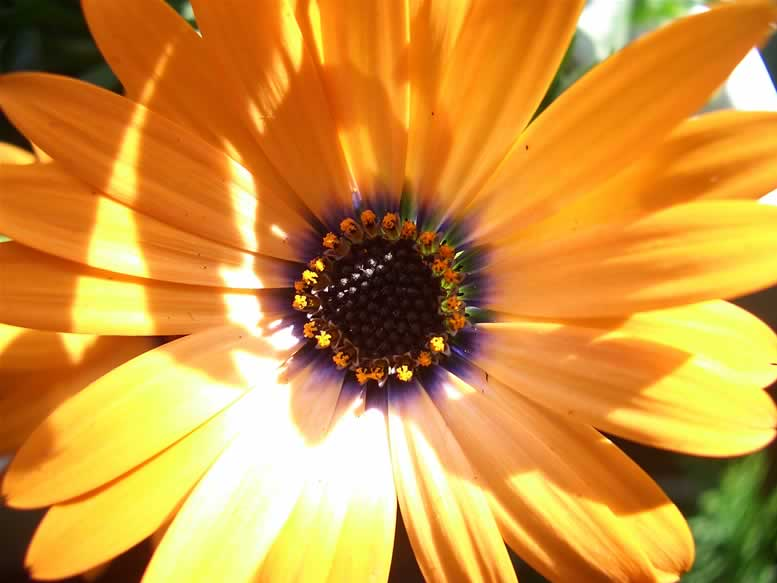
\includegraphics[width=\linewidth]{bilder/blume-beispielbild.jpg}
	\caption{bildunterschrift}
	
	Ein ganz ganz langer text zum bild\\
	kdfnakgflkadshfkjsfkljsadfjk�adshf�lkdf\\
	hsgkj�ldhflkghsfdlkgh�dklfhglkdsjgl�dshgkdsfh�gh\\
	sdflkendgkjhdsfk�ghadfsopfghaoifhaigtfuiaerhgiuag
\newpage

\end{figure}

\begin{figure}
\subsection{name des bildes}
	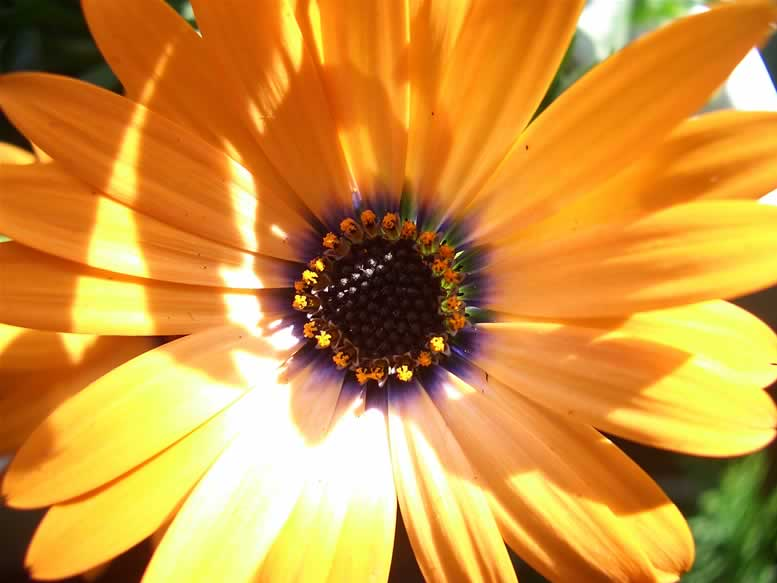
\includegraphics[width=\linewidth]{bilder/blume-beispielbild.jpg}
	\caption{bildunterschrift}
	
	Ein ganz ganz langer text zum bild\\
	kdfnakgflkadshfkjsfkljsadfjk�adshf�lkdf\\
	hsgkj�ldhflkghsfdlkgh�dklfhglkdsjgl�dshgkdsfh�gh\\
	sdflkgkjhdsfk�ghadfsopfghaoifhaigtfuiaerhgiuag
\newpage

\end{figure}
	

\chapter{Messagetypes}

\section{HostStatistics}
\lstinputlisting{./messagetypes/HostStatistics.msg}

\newpage

\section{NodeStatistics}
\lstinputlisting{./messagetypes/NodeStatistics.msg}

\newpage
\section{RatedStatistics}
\lstinputlisting{./messagetypes/RatedStatistics.msg}


\section{RatedStatisticsEntity}
\lstinputlisting{./messagetypes/RatedStatisticsEntity.msg}
\chapter{Servicetypes}

\section{NodeReaction}
\lstinputlisting{./messagetypes/NodeReaction.srv}

\section{StatisticHistory}
\lstinputlisting{./messagetypes/StatisticHistory.srv}


\chapter{Sequence diagrams}

\section{Dataprocessing and -storage}
\begin{figure}[!ht]
	\begin{center}
		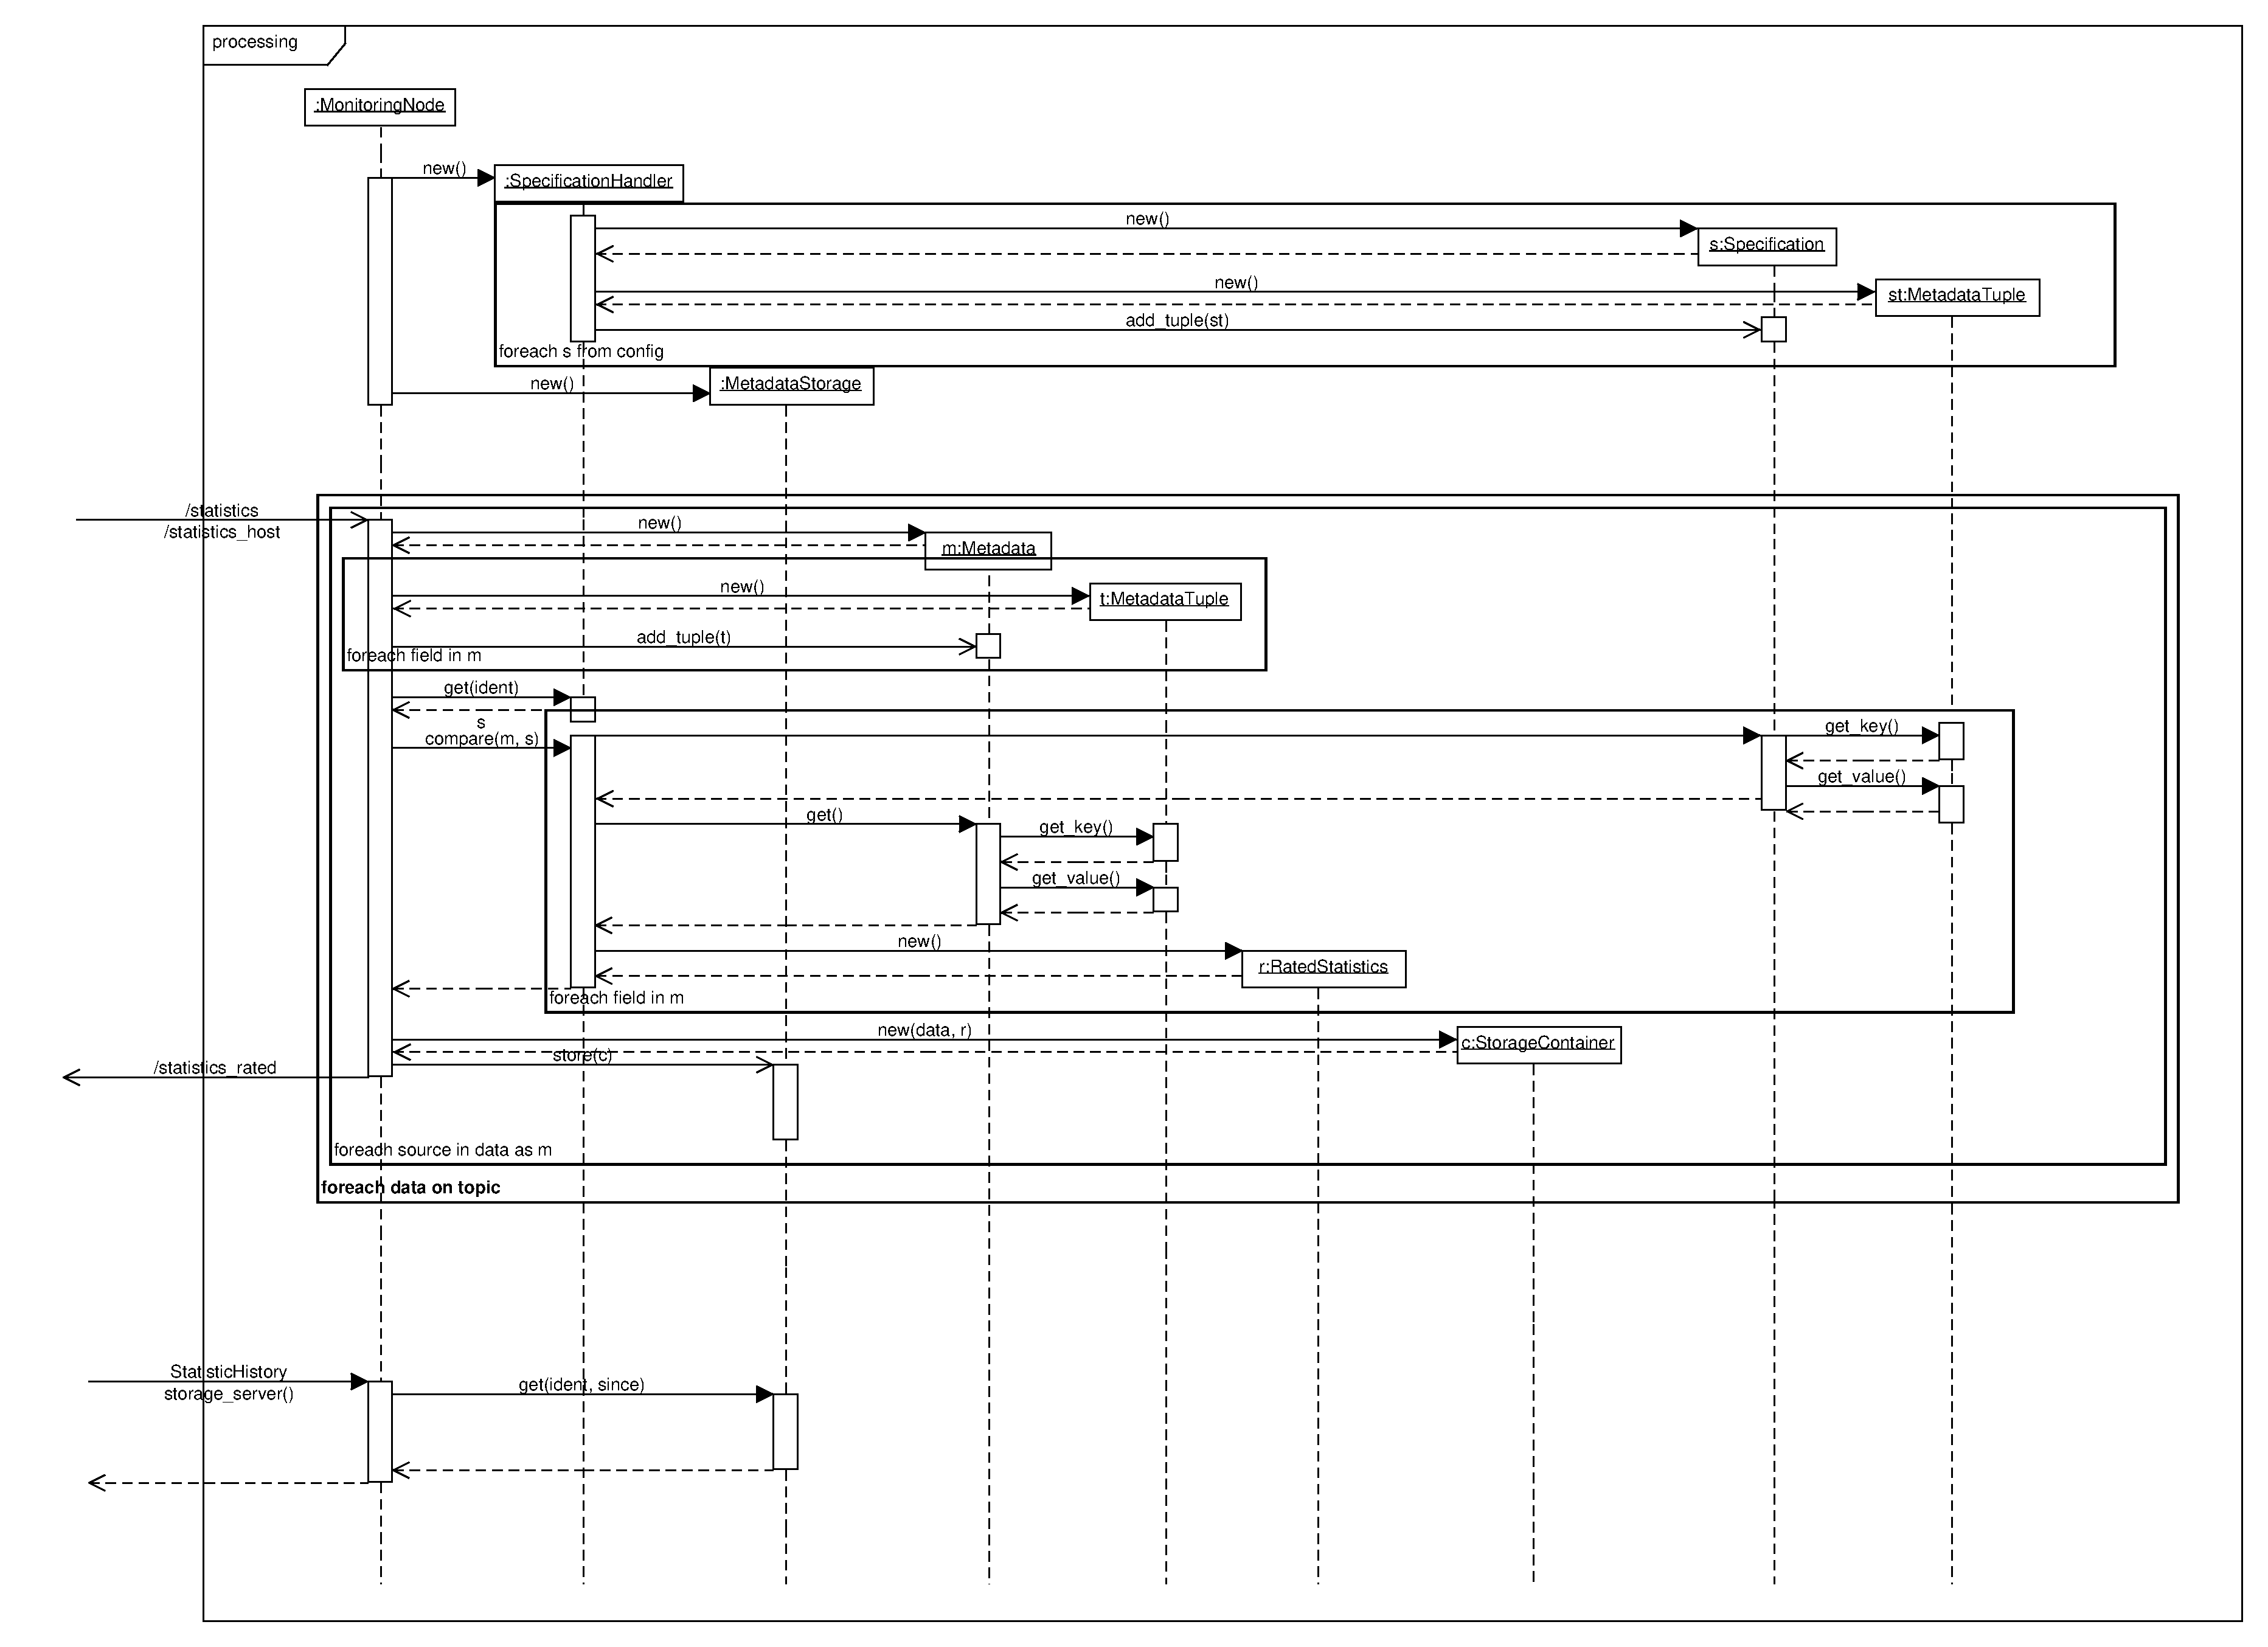
\includegraphics[width=1.0\linewidth]{./diagram_pictures/processing_seq.pdf}
		\caption{Three sequences appearing in the data-processing part of the project.}
	\end{center}
\end{figure}

\subsection*{Setup}
During the first activity of the MonitoringNode, it sets up a SpecificationHandler, which then loads all specifications from config files and stores them in MetadataTuple objects bundled in Specification objects.\\
It then sets up the MetadataStorage.

\subsection*{Receiving data}
The second activity of the MonitoringNode is triggered on receiving data on either the /statistics or /statistics\_host topic. The incoming data is translated into Metadata objects containing of several MetadataTuples describing every measurement featured in the received data.\\
Now the MonitoringNode looks up a Specification from SpecificationHandler concerning the connection/node/host it just received data about.\\
On success it compares the created Metadata object with the found Specification object MetadataTuple-wise for each field featured in the Metadata/Specification object.\\
Erroneous results will be marked in a new RatedStatistics object. Bundled with the raw input data, a timestamp and an identifier describing the concerned connection/node/host it will be stored in the MetadataStorage object created on setup.

\subsection*{Providing data for the GUI}
Answering a request for all data or a special identifier describing a connection/node/host since a given point of time, the MonitoringNode will return the matching data from the MetadataStorage.
A result of that will contain raw data, rated data, a timestamp and the identifier mentioned above.

<<<<<<< HEAD
\section{GUI}
\begin{figure}[!ht]
	\begin{center}
		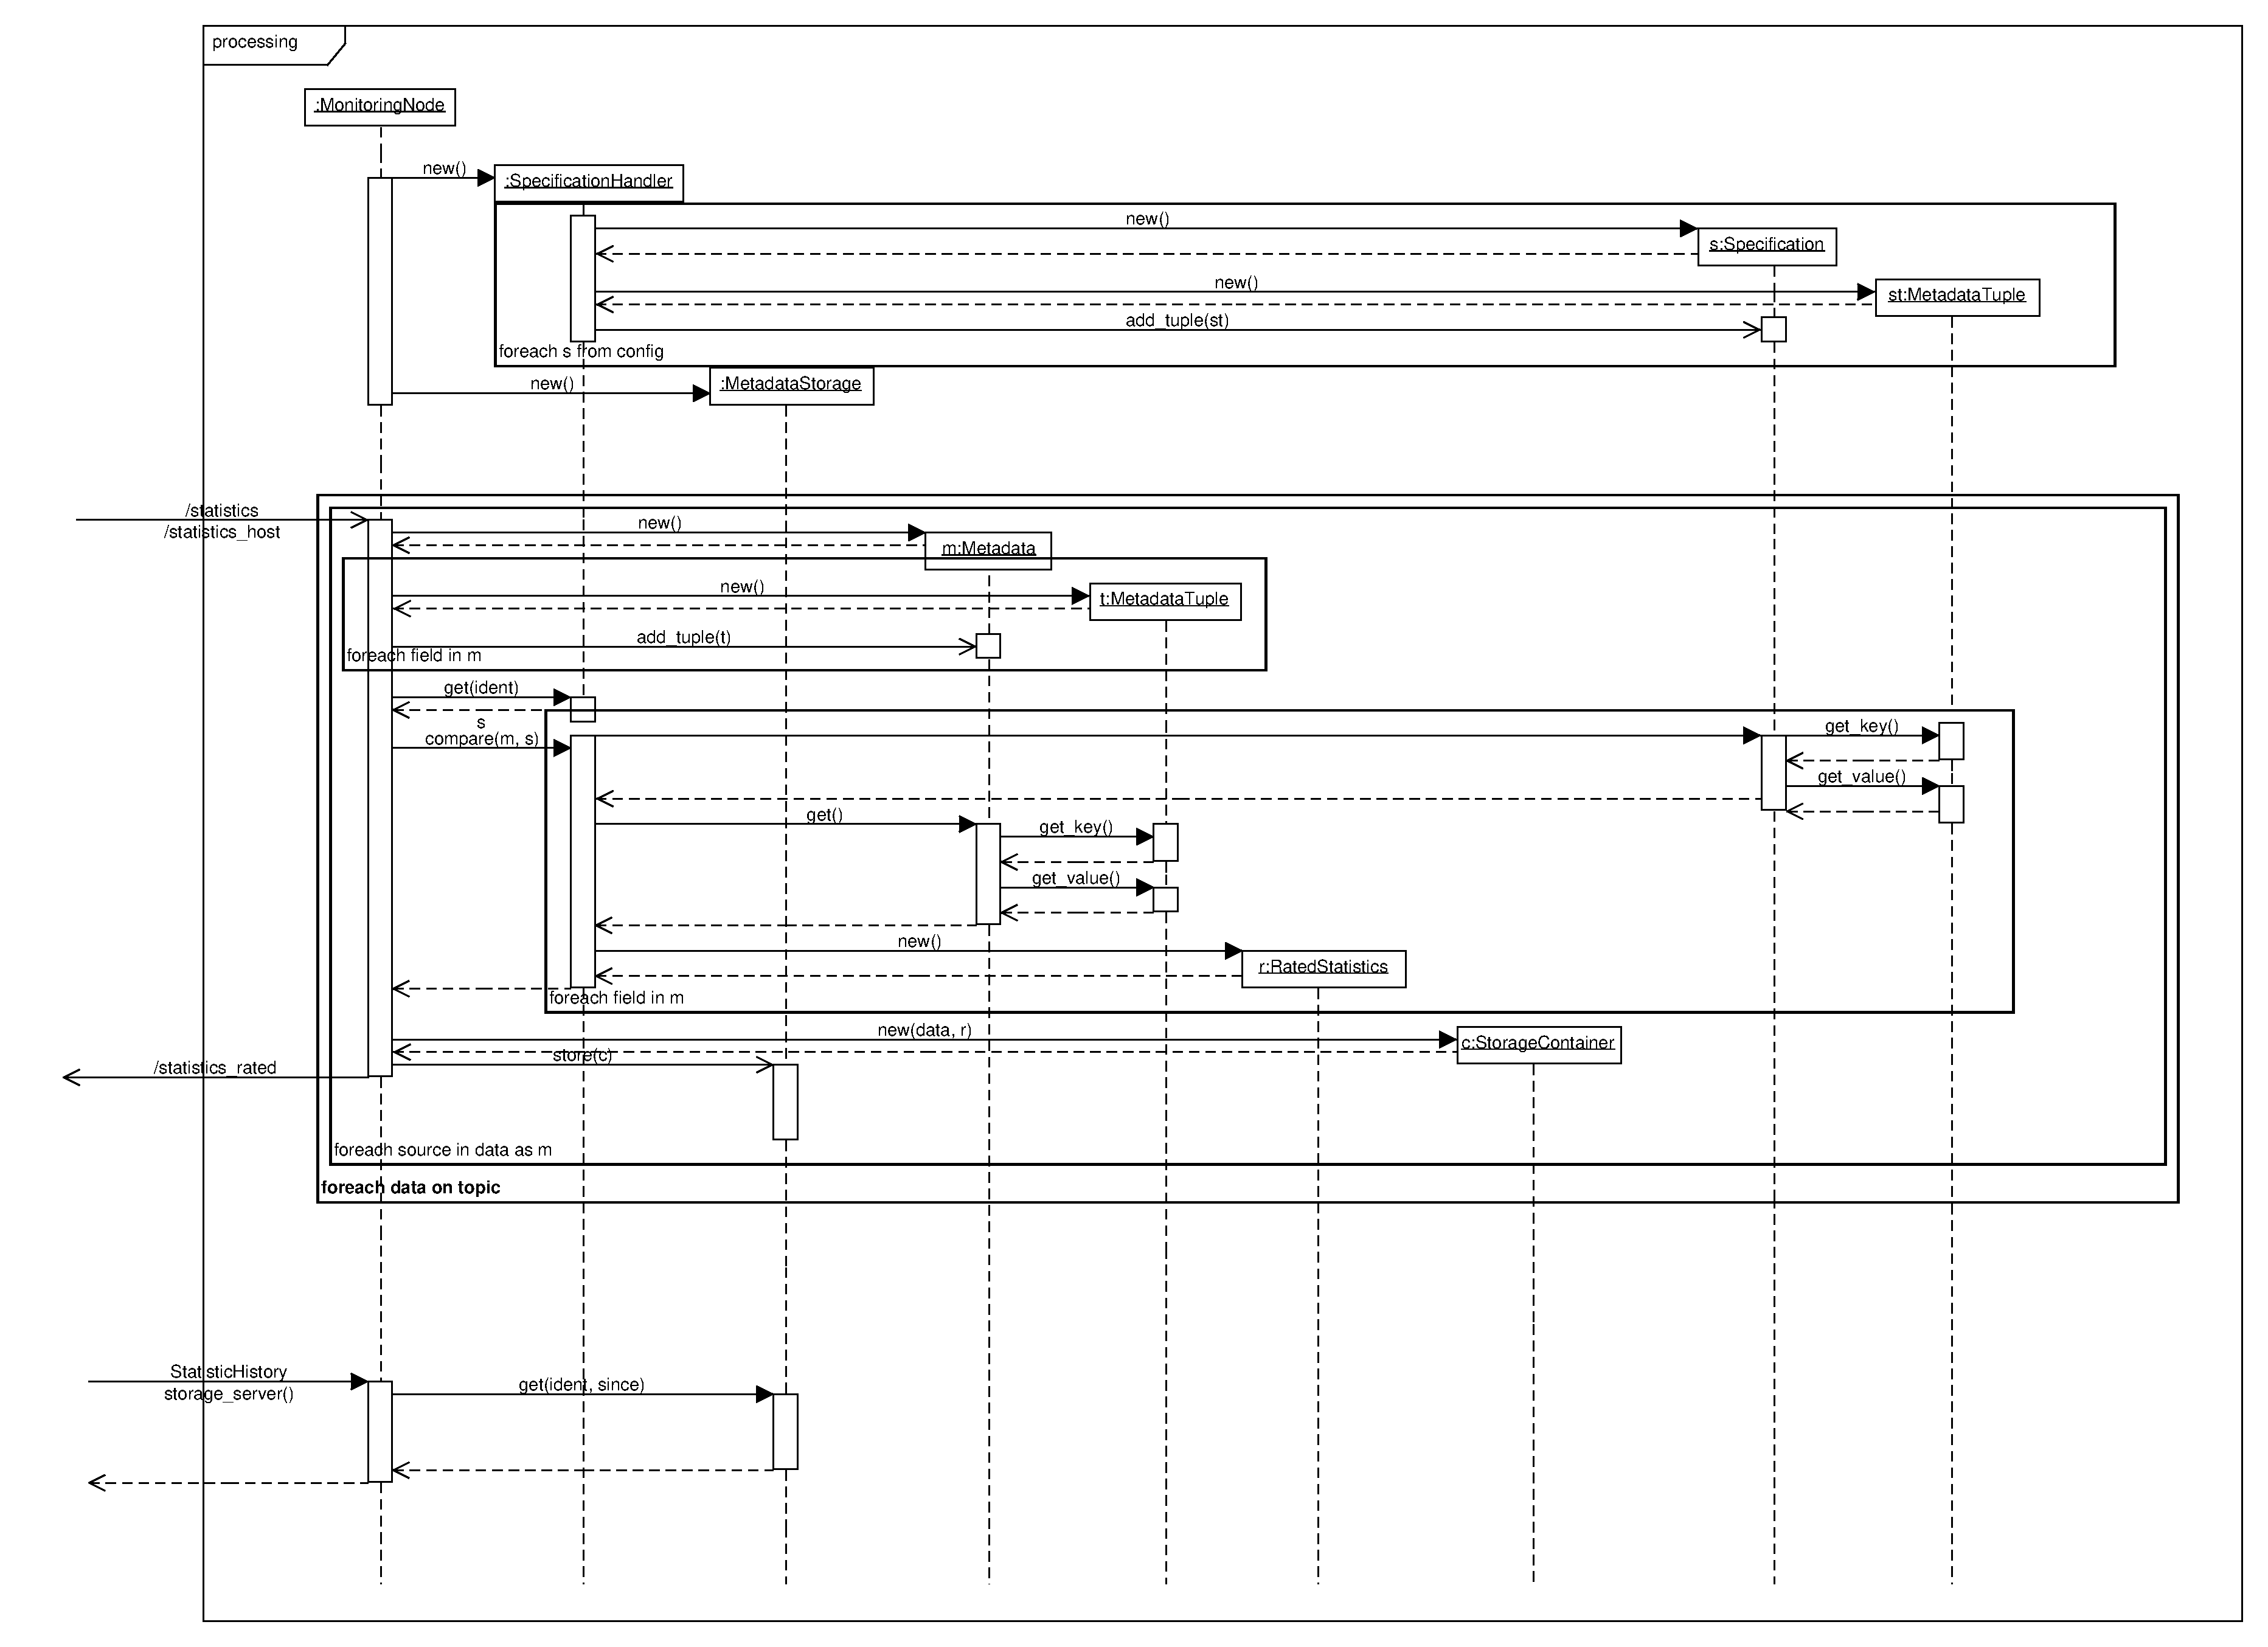
\includegraphics[width=1.0\linewidth]{./diagram_pictures/processing_seq.pdf}
		\caption{Three sequences appearing in the data-processing part of the project.}
	\end{center}
\end{figure}
\subsection{Setup}
In this sequence diagramm it is exemplary shown how the GUI part of the Software initializes.
All widgets do whenever startet proceed the following steps: Initialize their own data, create or get the model, synchronize with an additional proxy model and then create and start the BufferThread so data is flowing in. The BufferThread then connects via the services to the MonitoringNode and gets a history of the last messages.
Finally the widgets connect their slots so that e.g. the view gets updated when the model changes.
\subsection{Running}
When the GUI is running everything is getting updated with Qt's signal and slot mechanism. The BufferThread gets all actual data as a Subscriber of all topics and then regularily redirects this data by updating the model. The changes are then transmitted to the view aka the widgets which then show this incoming data.
\\
\\Any other information on how the classes work and interact can often be discovered by looking at the class diagram.
=======


\newpage
\section{Countermeasures}
\begin{figure}[!ht]
	\begin{center}
		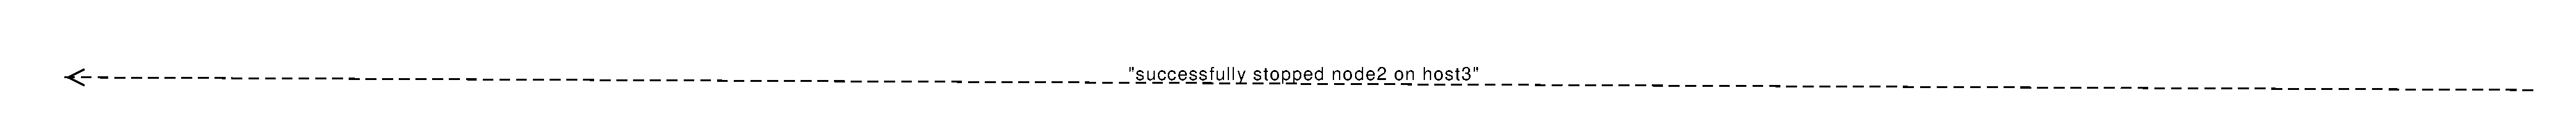
\includegraphics[width=1.0\linewidth]{./diagram_pictures/reactor/reactor_seq.pdf}
		\caption{Initialisation of Constraints and evaluating and executing countermeasures.}
	\end{center}
\end{figure}
>>>>>>> origin/master

\include{content/designdata}
\include{content/index}
\include{content/attachment}
\include{content/glossary}

\end{document}